\section{Reglervalidierung} \label{sec:Reglervalidierung}

\subsection{Validierung des linearen Modells} \label{sec:Vergleich_linear}

\subsubsection{Zustandsregler mit einfacher Zustandsrückführung}

\begin{figure}[H]
    \centering
    \fbox{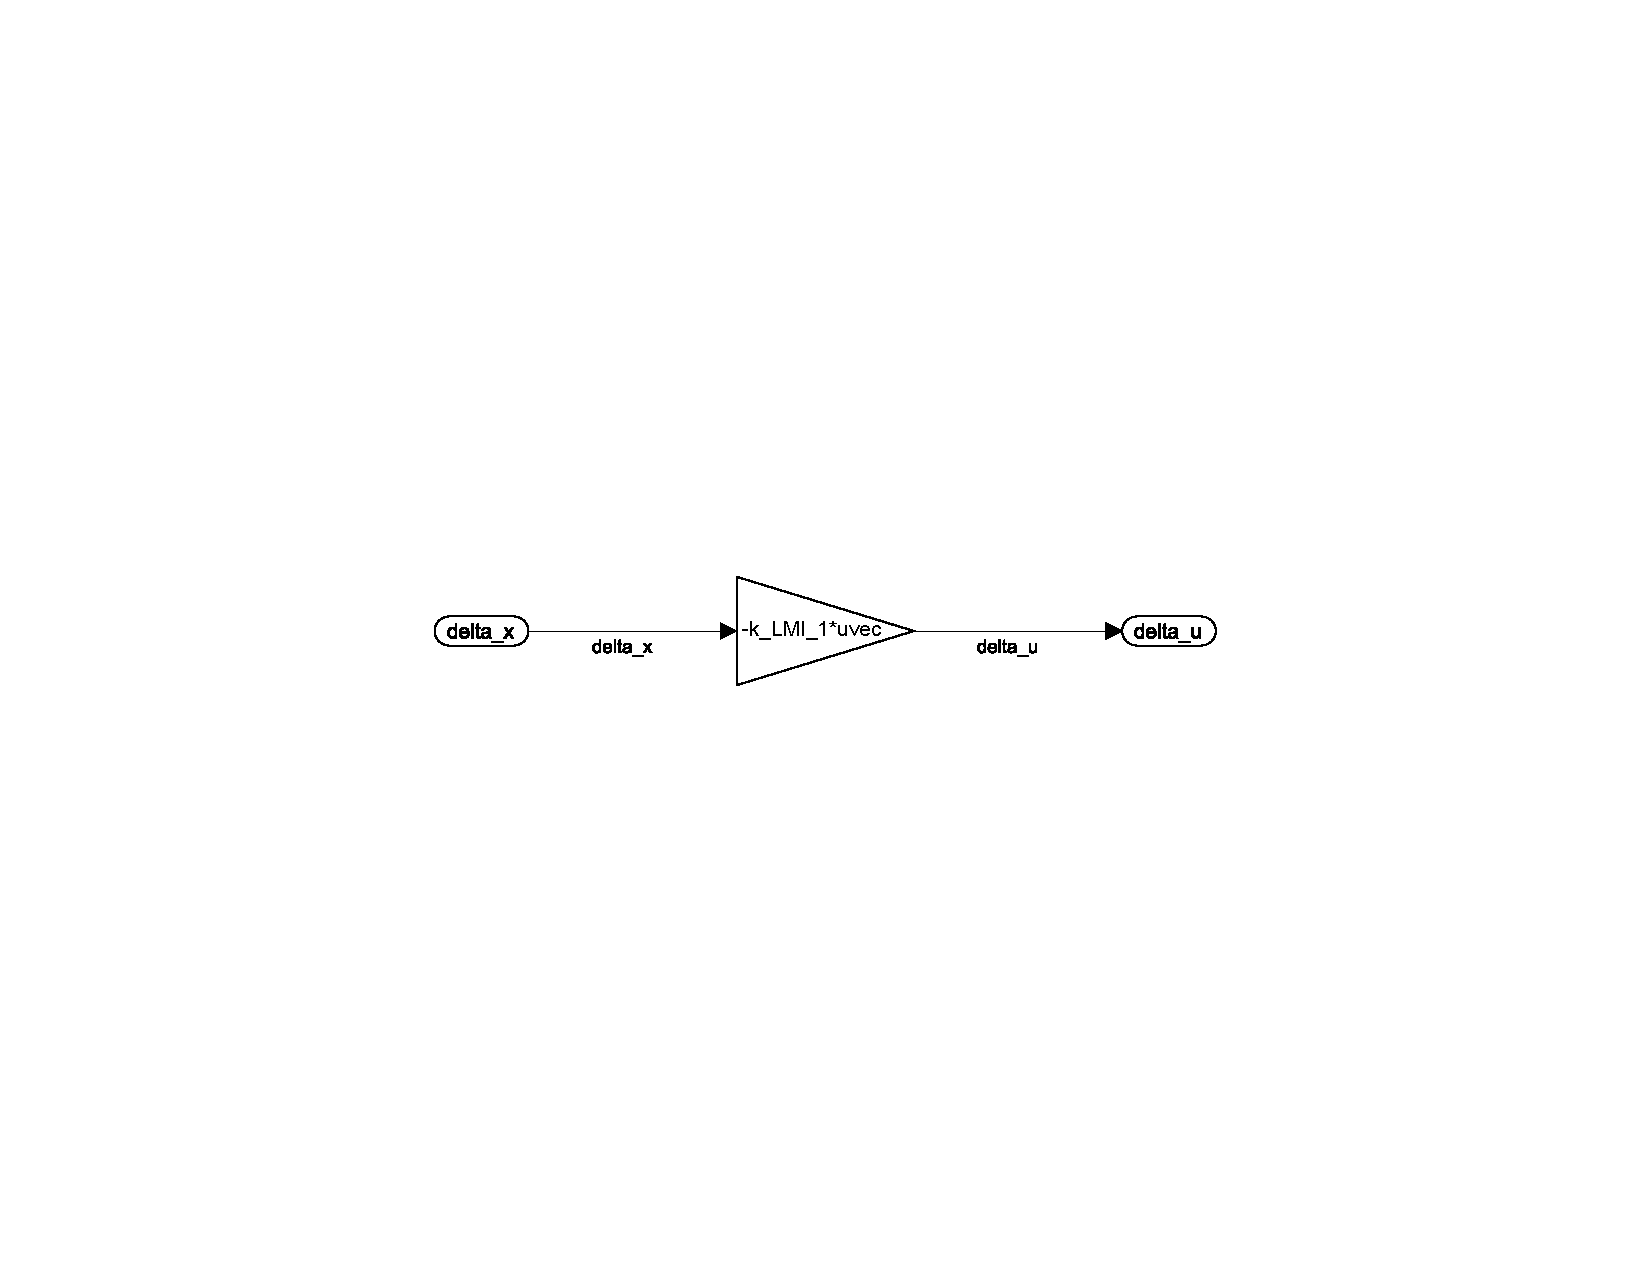
\includegraphics[width=0.7\textwidth]{Bilder/6_reglervalidierung/linear_einfacher_regler_simu.pdf}}
    \caption[Einfacher Zustandsregler Simulink (linear)]{Simulink Regler-Blockschaltbild für den einfachen Zustandsregler (lineares Zustandsraummodell)}
    \label{fig:Bild13}
\end{figure}

\begin{figure}[H]
    \centering
    \fbox{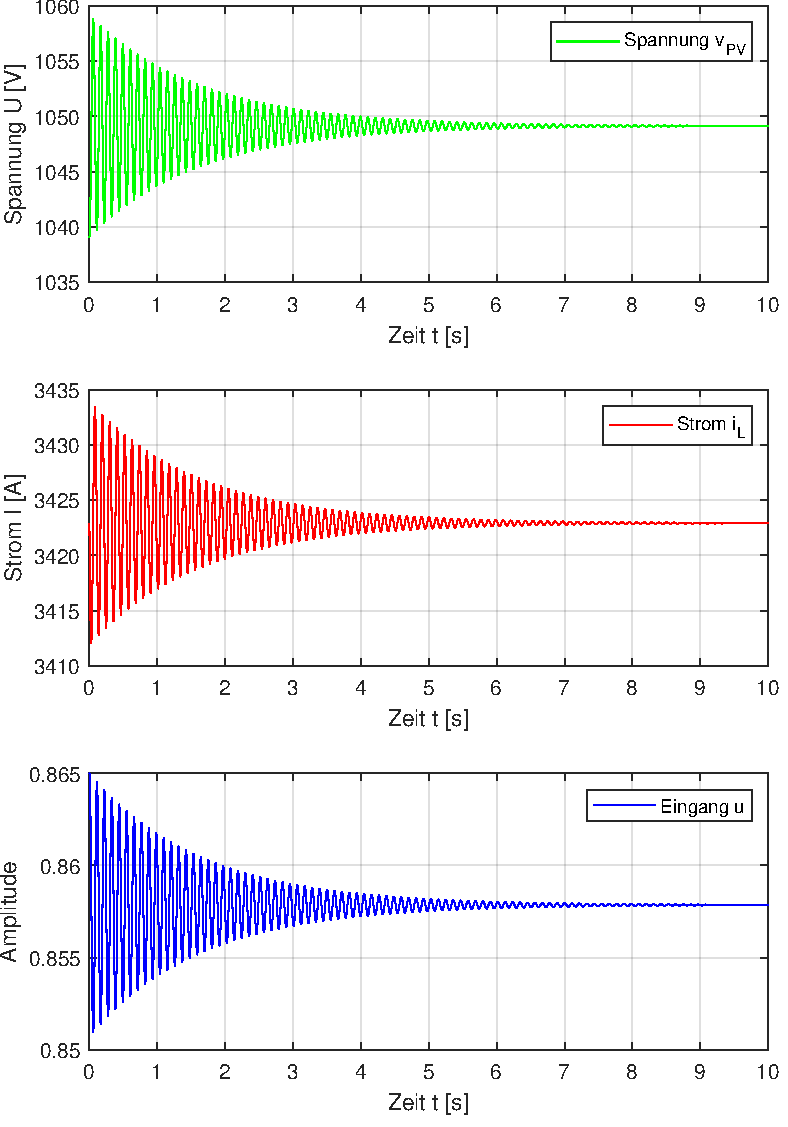
\includegraphics[width=0.85\textwidth]{Bilder/6_reglervalidierung/linear_einfache_rueckfuehrung.pdf}}
    \caption[Validierung Regler mit einfacher Rückführung (linear)]{$v_{\mathrm{PV}}$, $i_{\mathrm{L}}$ und $u$ bei einem Einganssprung von $v_{\mathrm{PV,MPP}} - \SI{10}{V}$ am einfachen Zustandsregler für das lineare Zustandsraummodell}
    \label{fig:Bild14}
\end{figure}

\subsubsection{Zustandsregler mit Vorsteuerung}

\begin{figure}[H]
    \centering
    \fbox{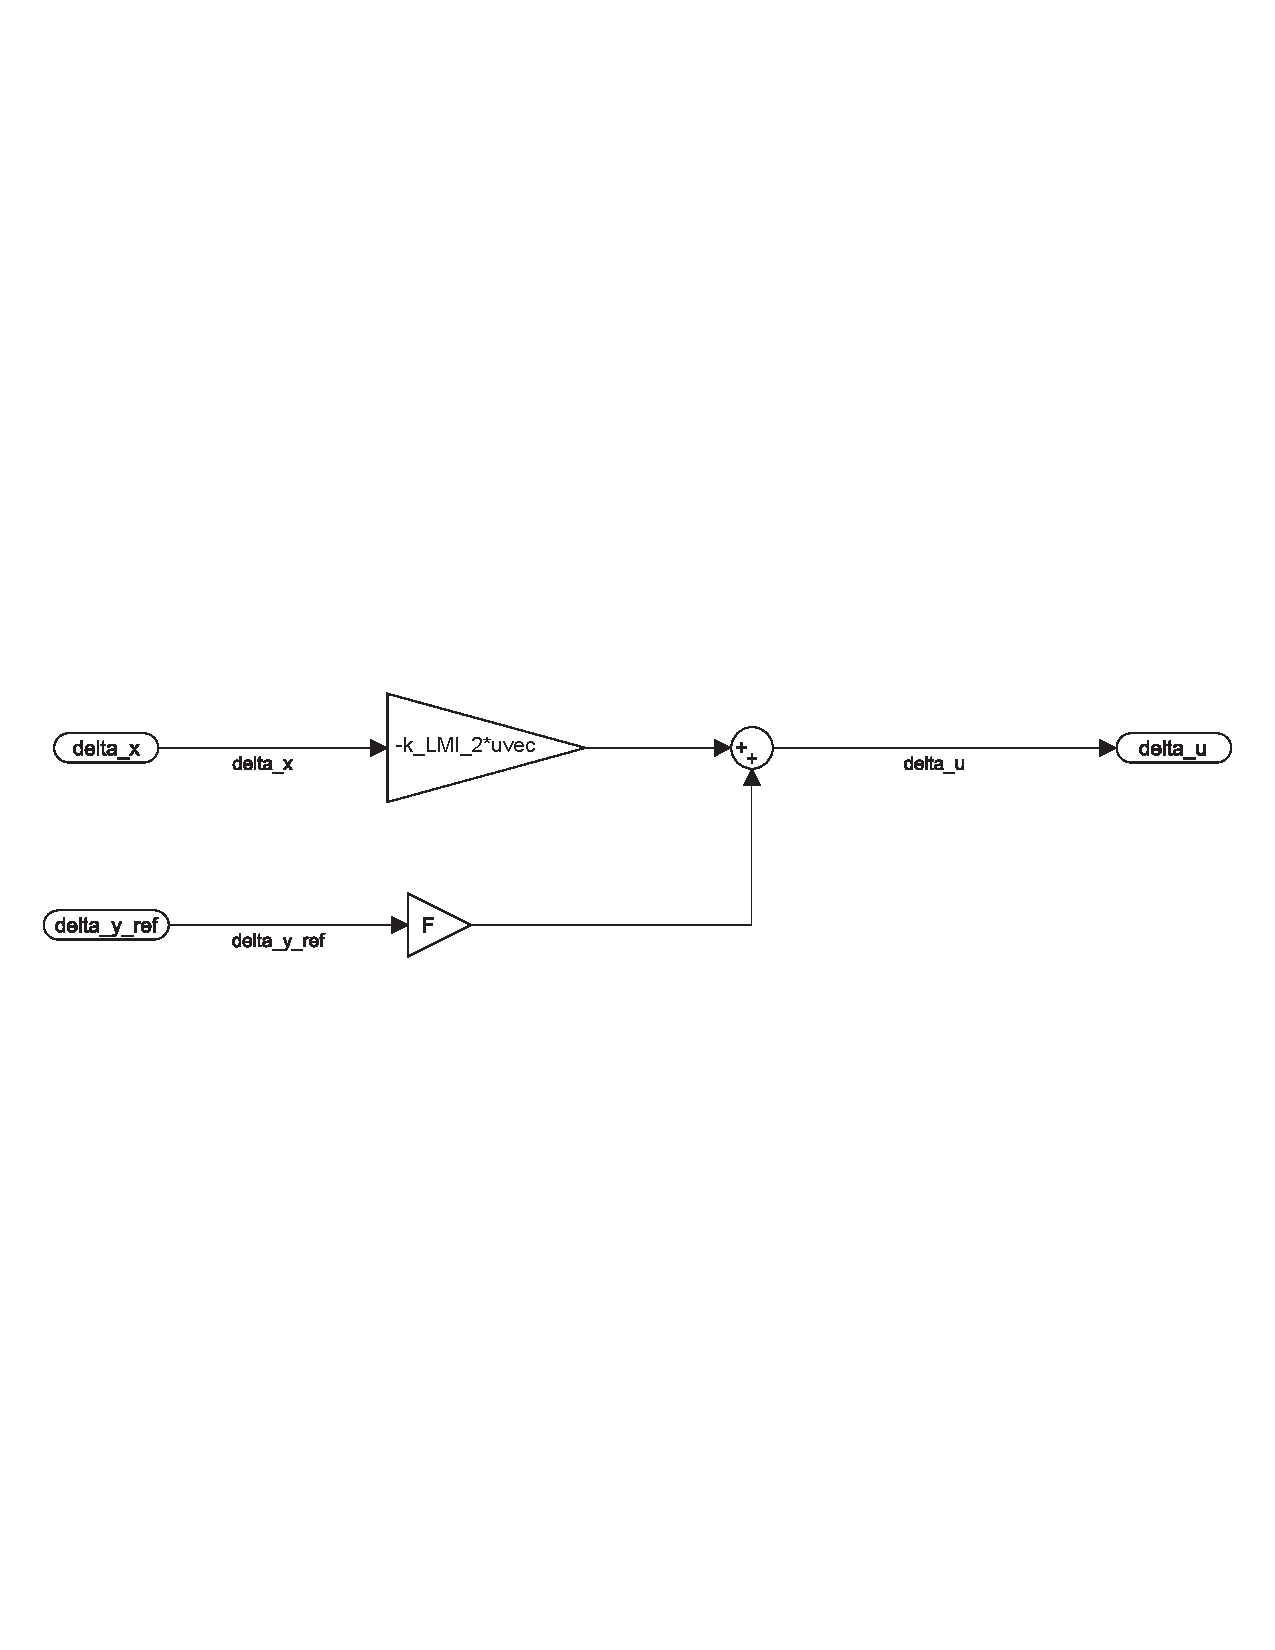
\includegraphics[width=1.0\textwidth]{Bilder/6_reglervalidierung/linear_vorsteuerung_simu.pdf}}
    \caption[Zustandsregler mit Vorsteuerung Simulink (linear)]{Simulink Regler-Blockschaltbild für den Zustandsregler mit Vorsteuerung (lineares Zustandsraummodell)}
    \label{fig:Bild15}
\end{figure}

\begin{figure}[H]
    \centering
    \fbox{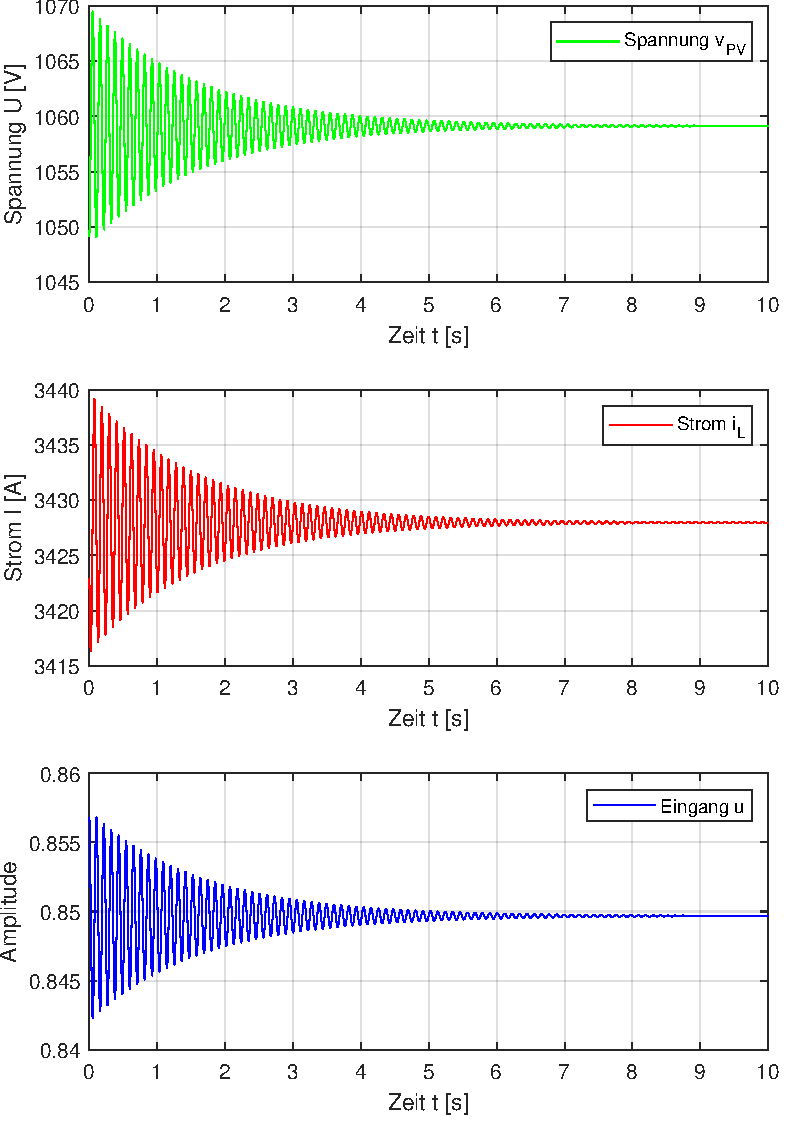
\includegraphics[width=0.85\textwidth]{Bilder/6_reglervalidierung/linear_referenzwertvorsteuerung.pdf}}
    \caption[Validierung Regler mit Vorsteuerung (linear)]{$v_{\mathrm{PV}}$, $i_{\mathrm{L}}$ und $u$ bei einem Referenzwert von $y_{ref} = v_{\mathrm{PV,MPP}} + \SI{10}{V}$ am Zustandsregler mit Referenzwertvorsteuerung für das lineare Zustandsraummodell}
    \label{fig:Bild16}
\end{figure}

\subsubsection{Zustandsregler mit I-Regelung}

\begin{figure}[H]
    \centering
    \fbox{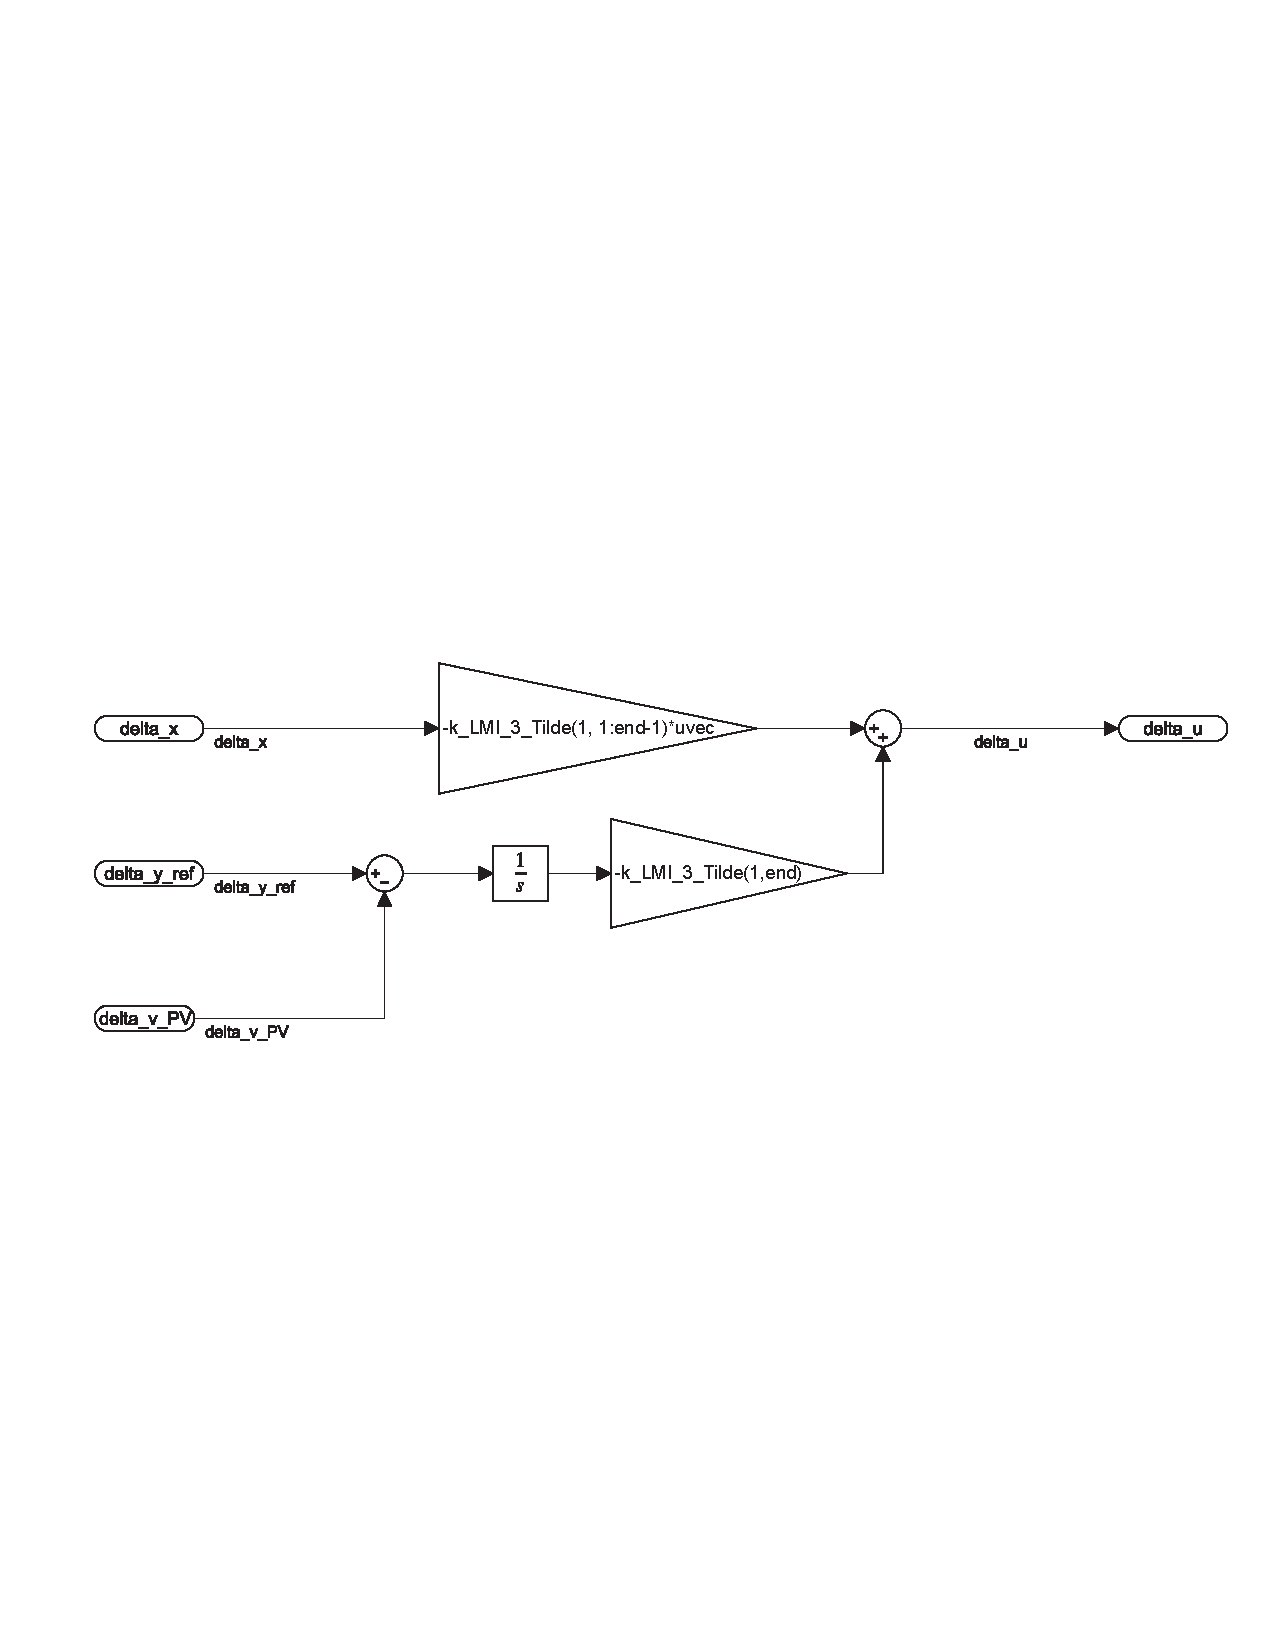
\includegraphics[width=1.0\textwidth]{Bilder/6_reglervalidierung/linear_i_regler_simu.pdf}}
    \caption[Zustandsregler mit I-Regelung Simulink (linear)]{Simulink Regler-Blockschaltbild für den Zustandsregler mit I-Regelung (lineares Zustandsraummodell)}
    \label{fig:Bild17}
\end{figure}

\begin{figure}[H]
    \centering
    \fbox{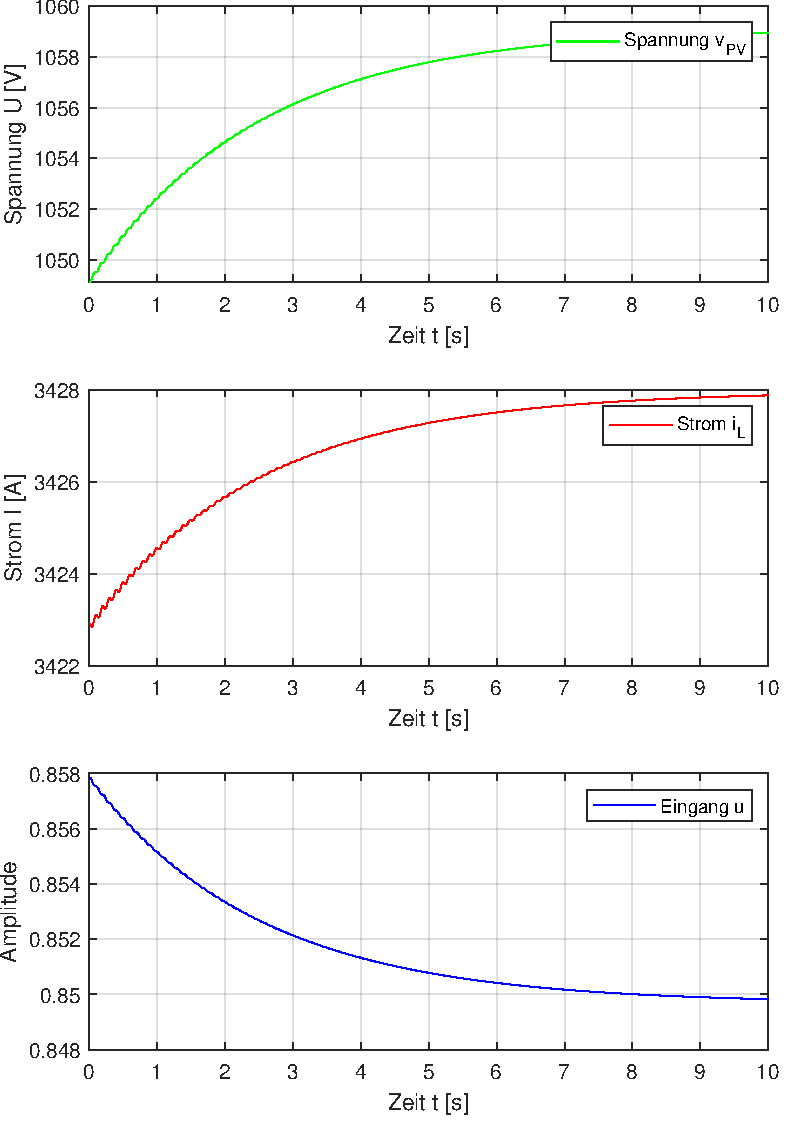
\includegraphics[width=0.85\textwidth]{Bilder/6_reglervalidierung/linear_i_regelung.pdf}}
    \caption[Validierung Regler mit I-Regelung (linear)]{$v_{\mathrm{PV}}$, $i_{\mathrm{L}}$ und $u$ bei einem Referenzwert von $y_{ref} = v_{\mathrm{PV,MPP}} + \SI{10}{V}$ am Zustandsregler mit I-Regelung für das lineare Zustandsraummodell}
    \label{fig:Bild18}
\end{figure}

\subsubsection{Vergleich des Regelverhaltens}

\begin{figure}[H]
    \centering
    \fbox{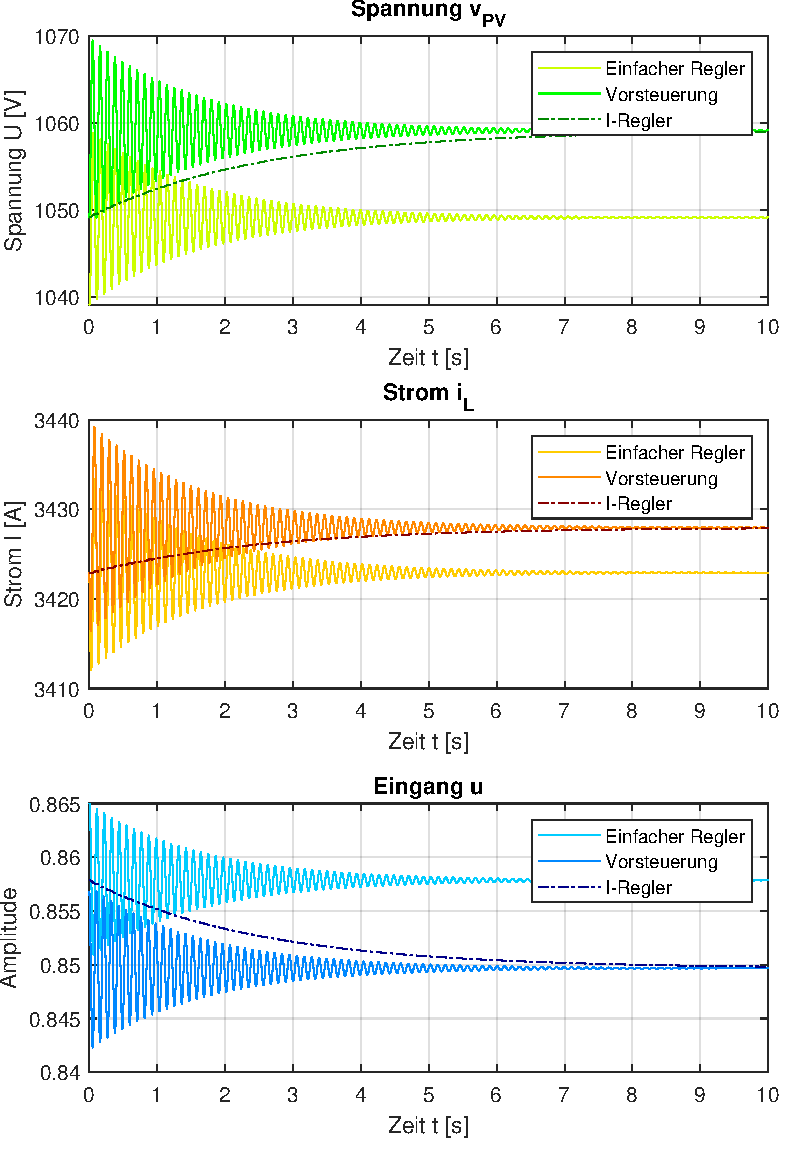
\includegraphics[width=0.7\textwidth]{Bilder/6_reglervalidierung/linear_reglervergleich.pdf}}
    \caption[Reglervergleich für das lineare Zustandsraummodell]{$v_{\mathrm{PV}}$, $i_{\mathrm{L}}$ und $u$ für Regler mit einfacher Zustandsrückführung, Regler mit Referenzwertvorsteuerung und Regler mit I-Regelung bei einem Einganssprung von $v_{\mathrm{PV,MPP}} - \SI{10}{V}$ \bzw einem Referenzwert von $y_{ref} = v_{\mathrm{PV,MPP}} + \SI{10}{V}$ am linearen Zustandsraummodell}
    \label{fig:Bild19}
\end{figure}

\subsection{Validierung des nichtlinearen Modells} \label{sec:Vergleich_nichtlinear}

\subsubsection{Zustandsregler mit einfacher Zustandsrückführung}

\begin{figure}[H]
    \centering
    \fbox{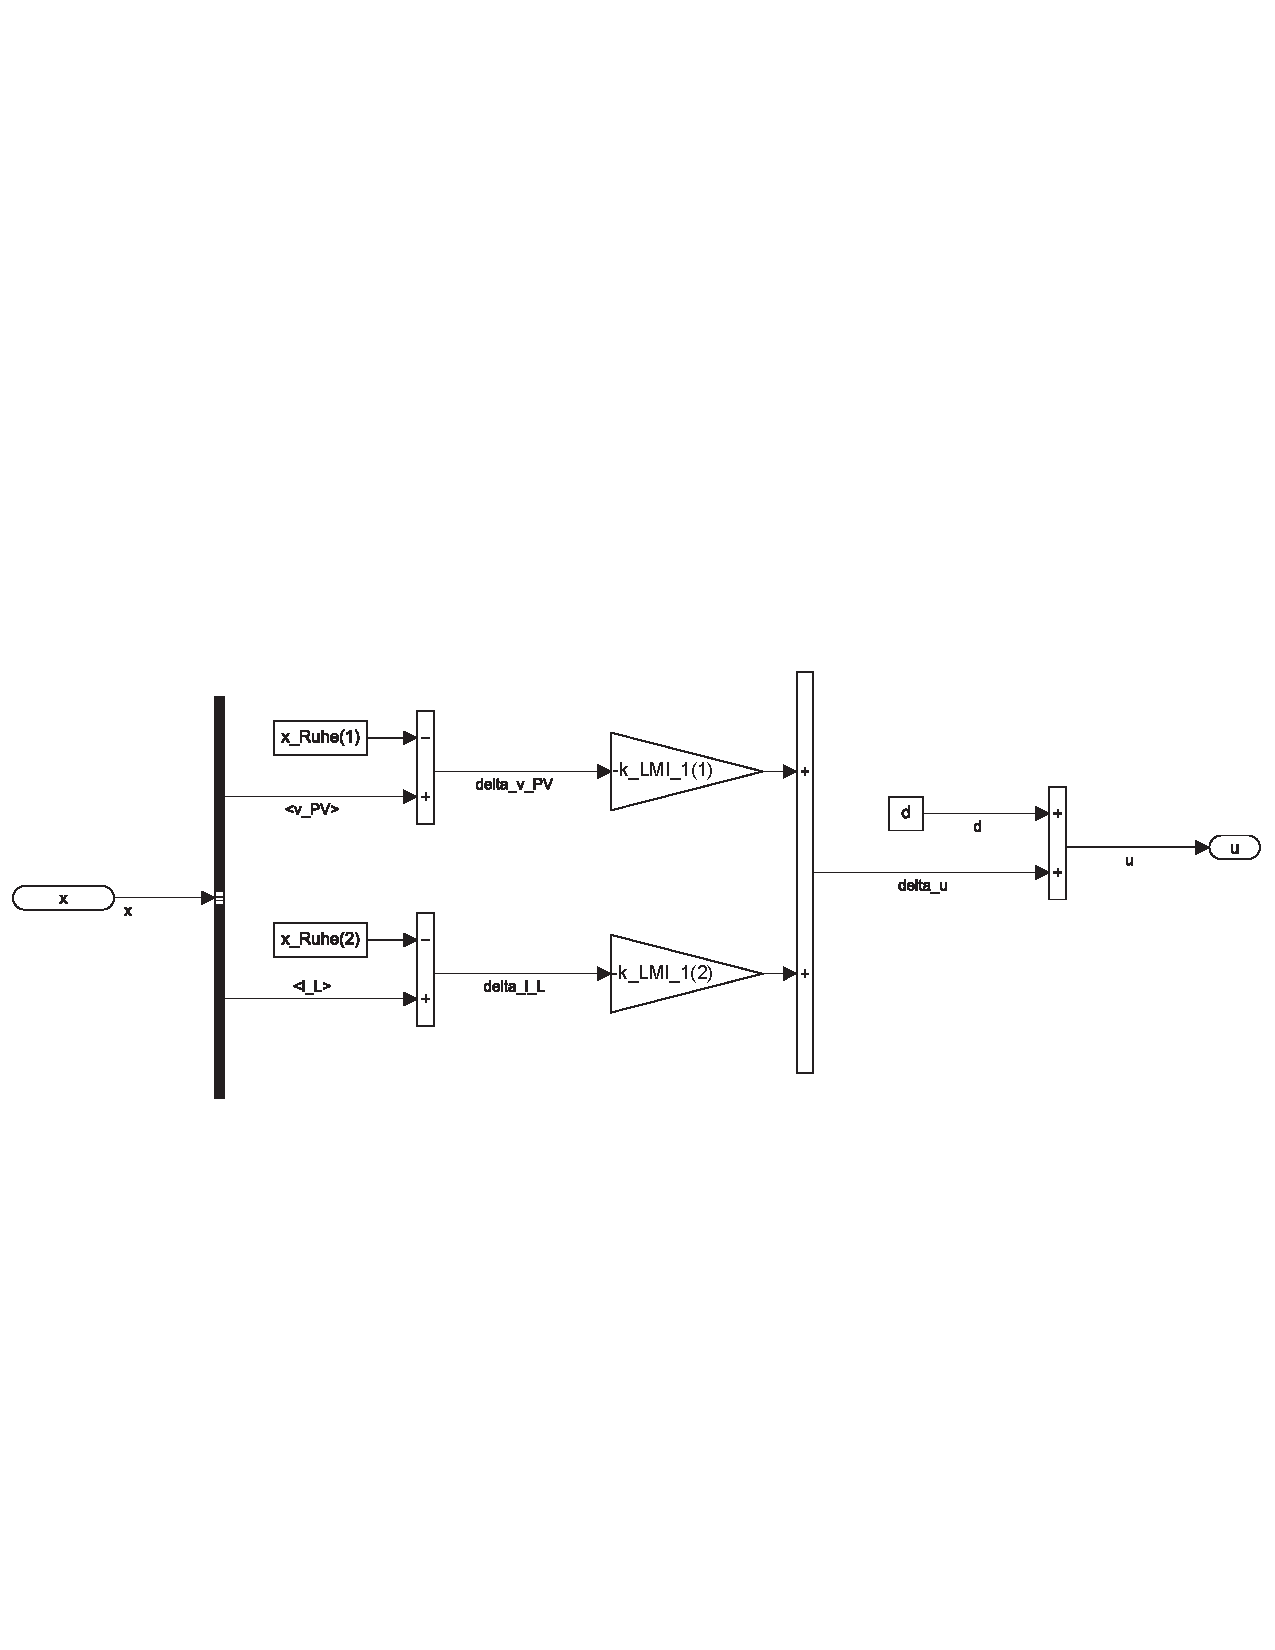
\includegraphics[width=1.0\textwidth]{Bilder/6_reglervalidierung/nichtlinear_einfacher_regler_simu.pdf}}
    \caption[Einfacher Zustandsregler Simulink (nicht-linear)]{Simulink Regler-Blockschaltbild für den einfachen Zustandsregler (nicht-lineares Zustandsraummodell)}
    \label{fig:Bild20}
\end{figure}

\begin{figure}[H]
    \centering
    \fbox{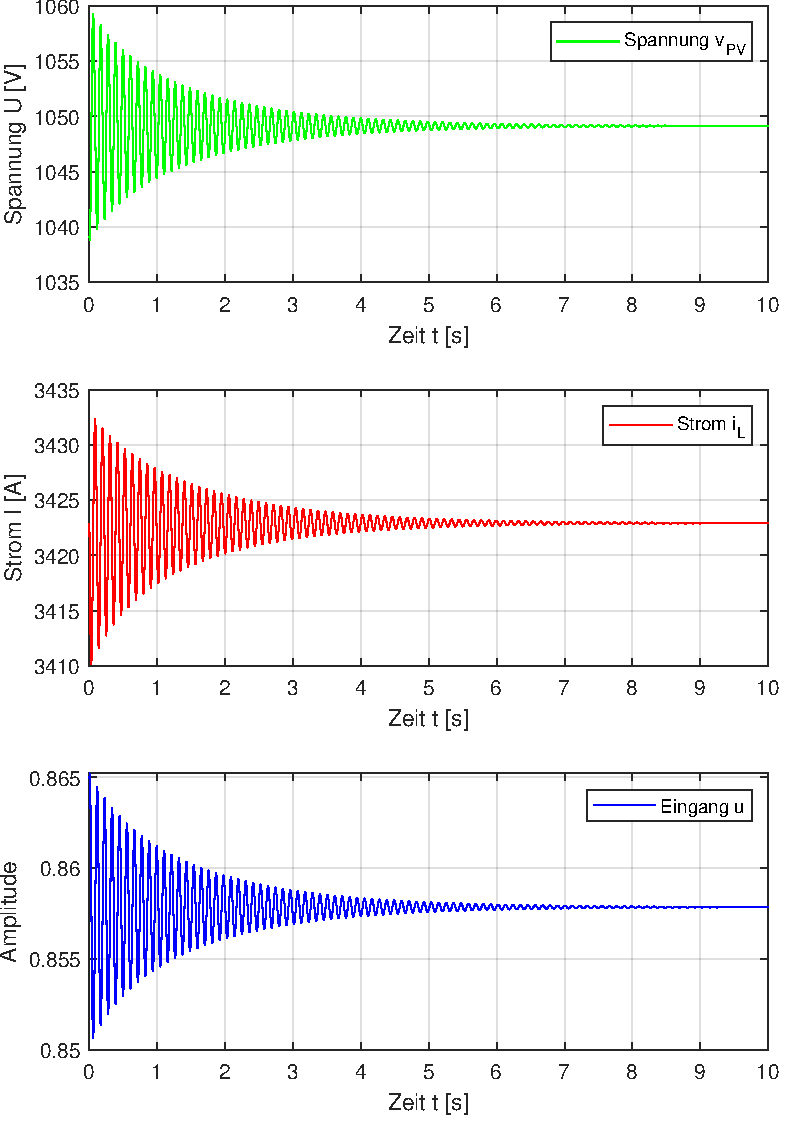
\includegraphics[width=0.85\textwidth]{Bilder/6_reglervalidierung/nichtlinear_einfache_rueckfuehrung.pdf}}
    \caption[Validierung Regler mit einfacher Rückführung (nicht-linear)]{$v_{\mathrm{PV}}$, $i_{\mathrm{L}}$ und $u$ bei einem Einganssprung von $v_{\mathrm{PV,MPP}} - \SI{10}{V}$ am einfachen Zustandsregler für das nicht-lineare Zustandsraummodell}
    \label{fig:Bild21}
\end{figure}

\subsubsection{Zustandsregler mit Vorsteuerung}

\begin{figure}[H]
    \centering
    \fbox{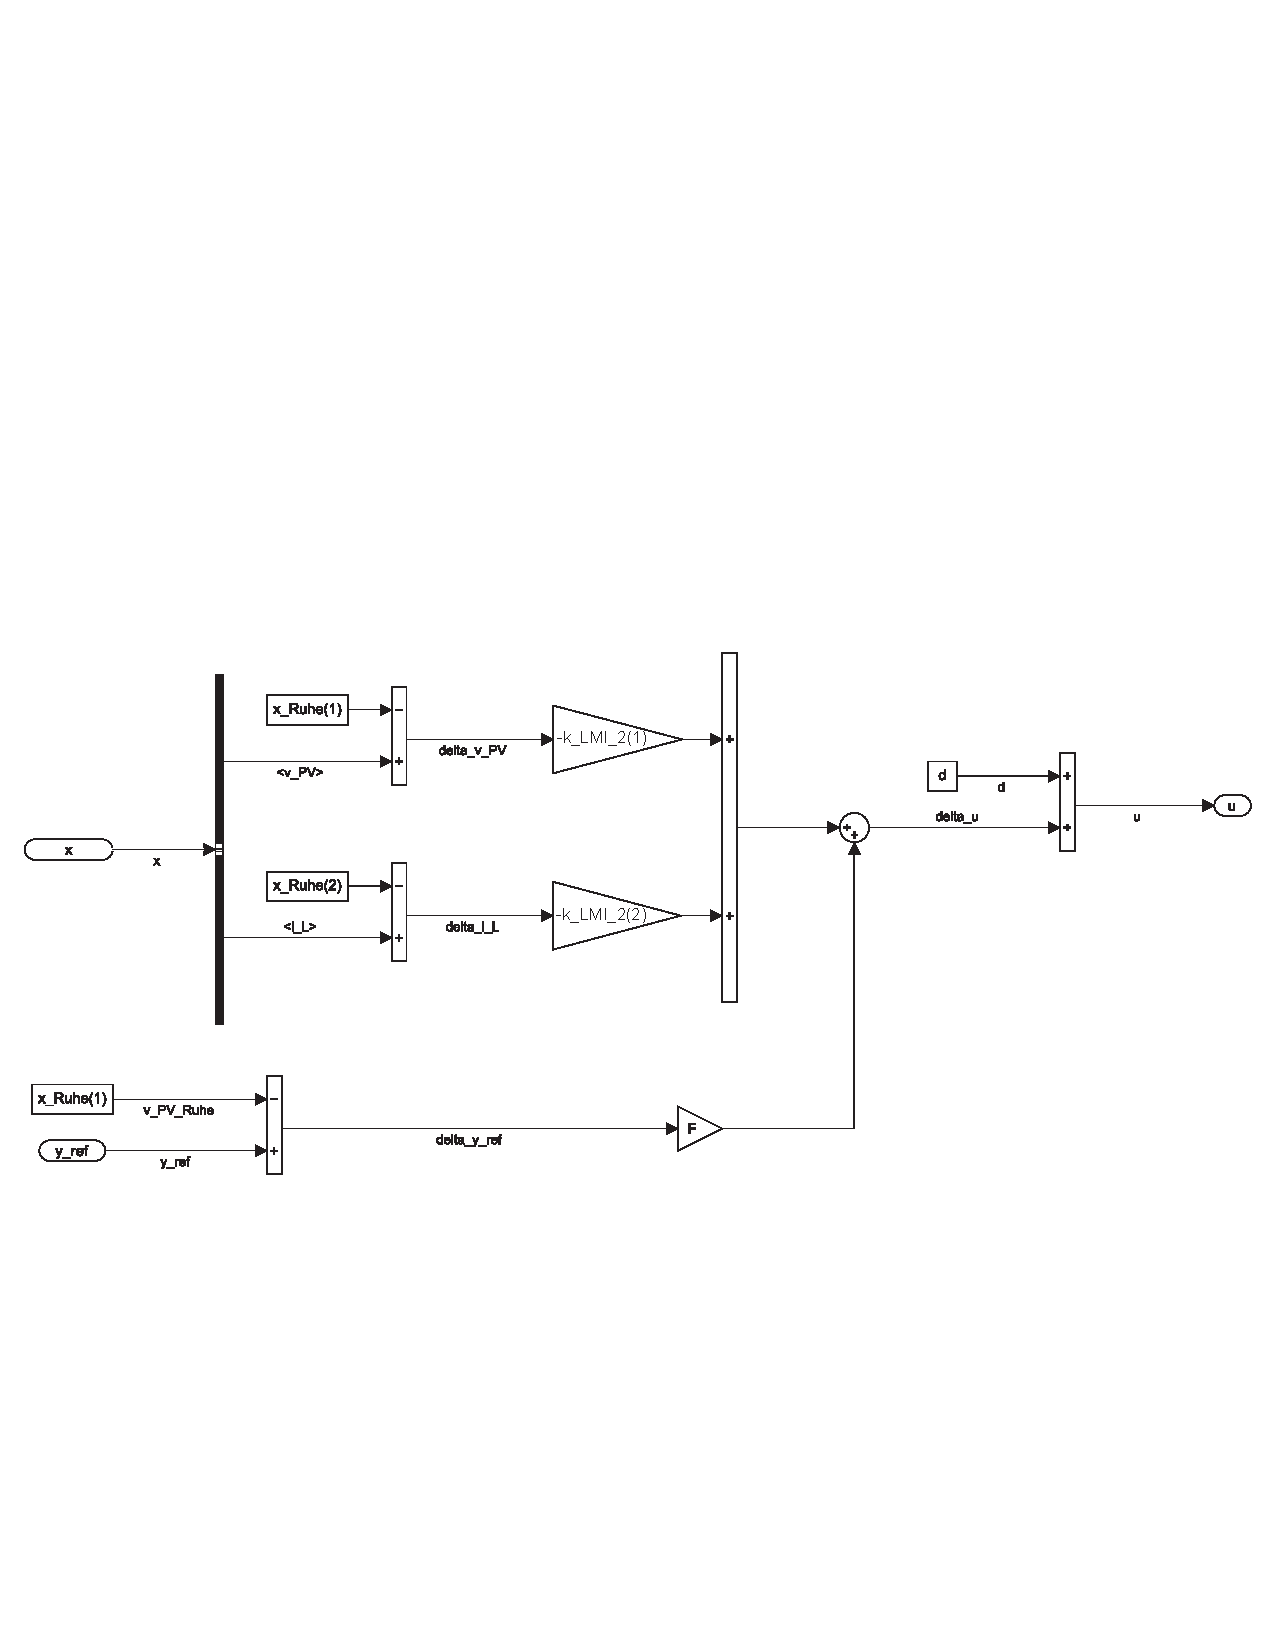
\includegraphics[width=1.0\textwidth]{Bilder/6_reglervalidierung/nichtlinear_vorsteuerung_simu.pdf}}
    \caption[Zustandsregler mit Vorsteuerung Simulink (nicht-linear)]{Simulink Regler-Blockschaltbild für den Zustandsregler mit Vorsteuerung (nicht-lineares Zustandsraummodell)}
    \label{fig:Bild22}
\end{figure}

\begin{figure}[H]
    \centering
    \fbox{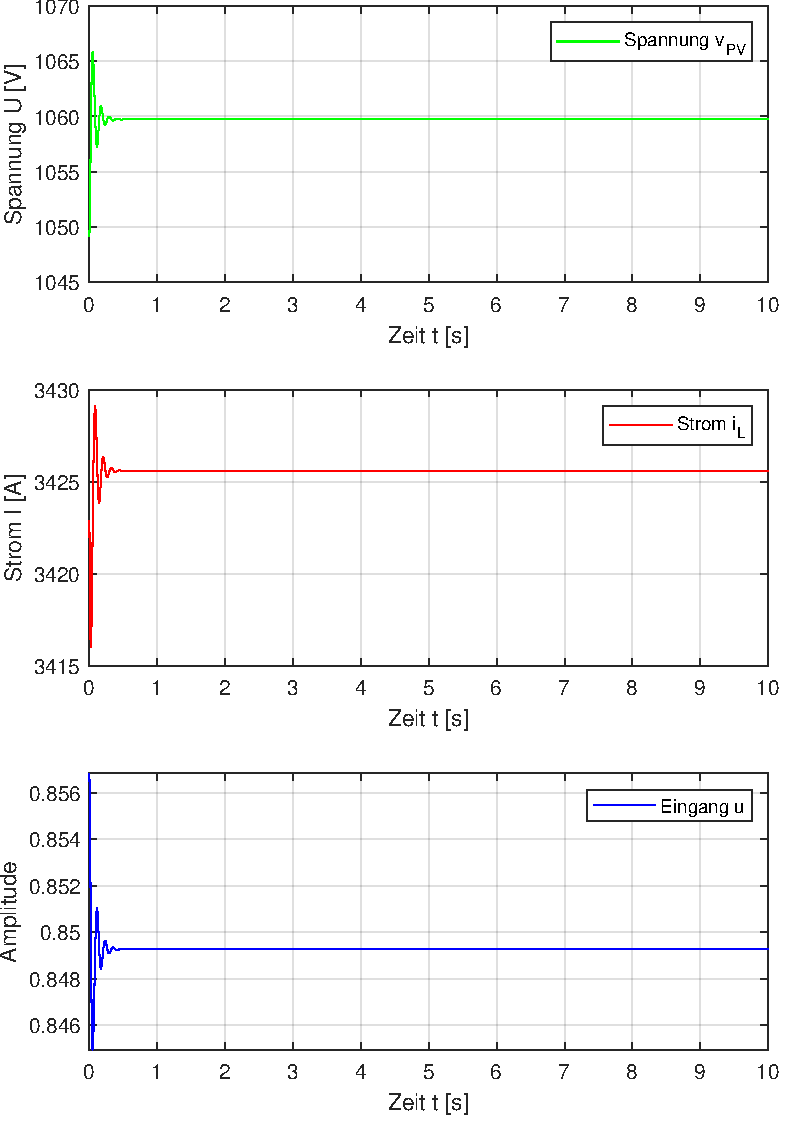
\includegraphics[width=0.85\textwidth]{Bilder/6_reglervalidierung/nichtlinear_referenzwertvorsteuerung.pdf}}
    \caption[Validierung Regler mit Vorsteuerung (nicht-linear)]{$v_{\mathrm{PV}}$, $i_{\mathrm{L}}$ und $u$ bei einem Referenzwert von $y_{ref} = v_{\mathrm{PV,MPP}} + \SI{10}{V}$ am Zustandsregler mit Referenzwertvorsteuerung für das nicht-lineare Zustandsraummodell}
    \label{fig:Bild23}
\end{figure}

\subsubsection{Zustandsregler mit I-Regelung}

\begin{figure}[H]
    \centering
    \fbox{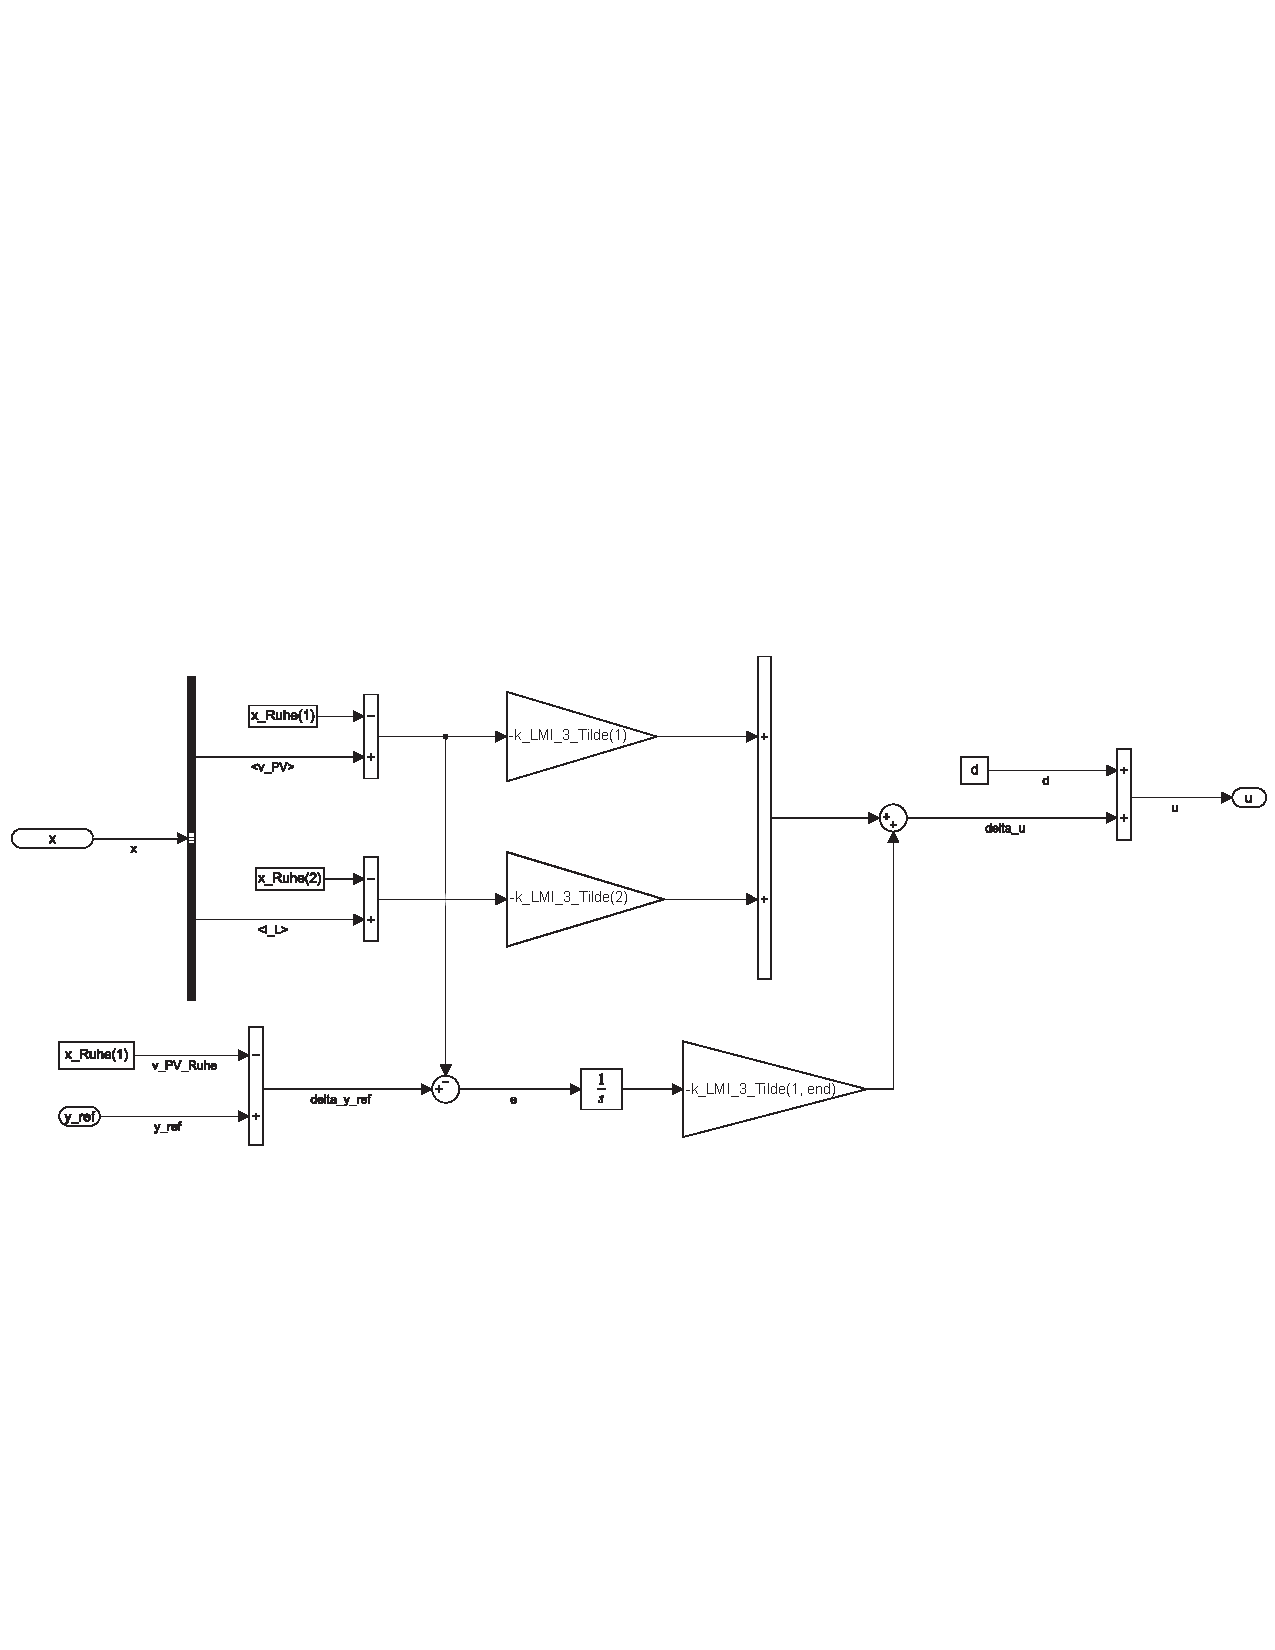
\includegraphics[width=1.0\textwidth]{Bilder/6_reglervalidierung/nichtlinear_i_regler_simu.pdf}}
    \caption[Zustandsregler mit I-Regelung Simulink (nicht-linear)]{Simulink Regler-Blockschaltbild für den Zustandsregler mit I-Regelung (nicht-lineares Zustandsraummodell)}
    \label{fig:Bild24}
\end{figure}

\begin{figure}[H]
    \centering
    \fbox{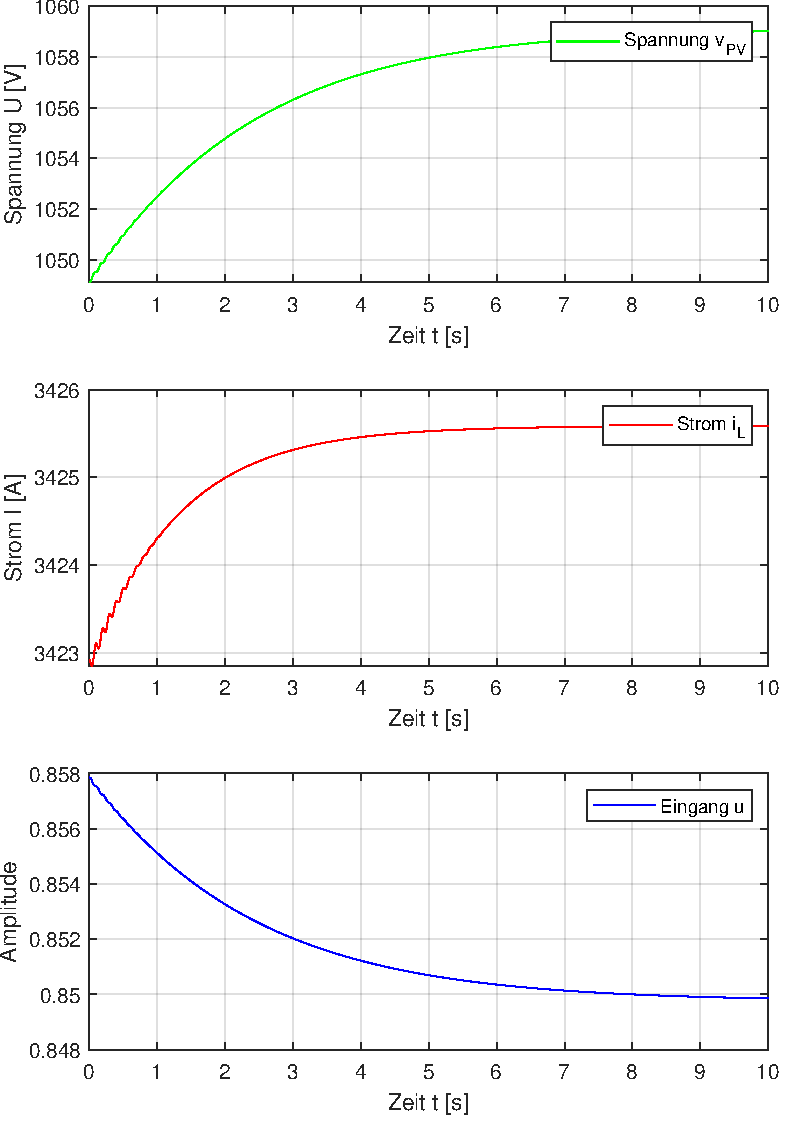
\includegraphics[width=0.85\textwidth]{Bilder/6_reglervalidierung/nichtlinear_i_regelung.pdf}}
    \caption[Validierung Regler mit I-Regelung (nicht-linear)]{$v_{\mathrm{PV}}$, $i_{\mathrm{L}}$ und $u$ bei einem Referenzwert von $y_{ref} = v_{\mathrm{PV,MPP}} + \SI{10}{V}$ am Zustandsregler mit I-Regelung für das nicht-lineare Zustandsraummodell}
    \label{fig:Bild25}
\end{figure}

\subsubsection{Vergleich des Regelverhaltens}

\begin{figure}[H]
    \centering
    \fbox{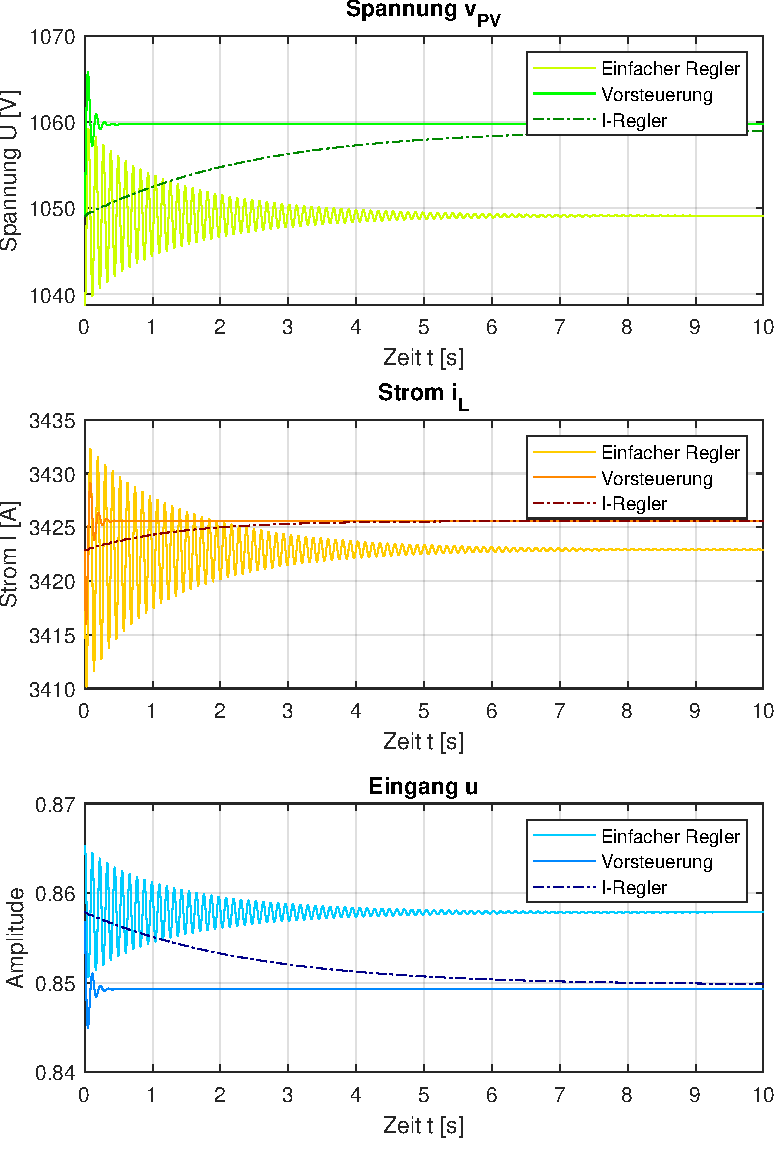
\includegraphics[width=0.7\textwidth]{Bilder/6_reglervalidierung/nichtlinear_reglervergleich.pdf}}
    \caption[Reglervergleich für das nicht-lineare Zustandsraummodell]{$v_{\mathrm{PV}}$, $i_{\mathrm{L}}$ und $u$ für Regler mit einfacher Zustandsrückführung, Regler mit Referenzwertvorsteuerung und Regler mit I-Regelung bei einem Einganssprung von $v_{\mathrm{PV,MPP}} - \SI{10}{V}$ \bzw einem Referenzwert von $y_{ref} = v_{\mathrm{PV,MPP}} + \SI{10}{V}$ am nicht-linearen Zustandsraummodell}
    \label{fig:Bild26}
\end{figure}